\documentclass[dvipdfmx,12pt]{jarticle}

\setlength{\oddsidemargin}{-0pt}
\setlength{\topmargin}{-20pt}
\setlength{\headheight}{-0pt}
\setlength{\headsep}{15pt}
\setlength{\textwidth}{16cm}
\setlength{\textheight}{23.5cm}
\setlength{\footskip}{70pt}

%Package for page setting
\usepackage[toc,page]{appendix}
\usepackage{booktabs}
\usepackage{pdfpages}
\usepackage[toc,page]{appendix}
\renewcommand{\appendixtocname}{付録}
\renewcommand{\appendixpagename}{付録}

%Package for tables, graphs, program lists
\usepackage{graphicx,color}
\usepackage{pgfplots}
\pgfplotsset{width=6cm,compat=1.3}
\usepackage[labelformat=simple]{subcaption} % graph next to graph
\usepackage{longtable}
\usepackage{multirow}
\usepackage{multicol}
\usepackage{array}
\newcolumntype{P}[1]{>{\centering\arraybackslash}p{#1}}
\newcolumntype{M}[1]{>{\centering\arraybackslash}m{#1}}
\usepackage{chngcntr}
\usepackage{listings,jlisting}

%Package for detailed formatting
\usepackage{url}
\usepackage{amsmath}
\usepackage{enumitem}

%% Custom Set
\definecolor{OliveGreen}{cmyk}{0.64,0,0.95,0.40}
\definecolor{colFunc}{rgb}{1,0.07,0.54}
\definecolor{CadetBlue}{cmyk}{0.62,0.57,0.23,0}
\definecolor{Brown}{cmyk}{0,0.81,1,0.60}
\definecolor{colID}{rgb}{0.63,0.44,0}

\lstdefinestyle{c}{
language=c,
basicstyle=\footnotesize\ttfamily,
keywordstyle={\color{OliveGreen}},
keywordstyle={[2]\color{colFunc}},
keywordstyle={[3]\color{CadetBlue}},
commentstyle={\itshape\color{Brown}},
identifierstyle={\color{colID}},
stringstyle=\color{blue},
tabsize=4,
frame=tRBl,
numbers=left,
numberstyle={\ttfamily\small},
breaklines=true,
backgroundcolor={\color[gray]{.95}},
captionpos=t,
}

\renewcommand\thesubfigure{(\alph{subfigure})}

%New commands
\newcommand\doubleRule{\toprule\toprule}
\makeatletter	
%listing
\newcommand\inputcode[2][]{%
  \filename@parse{\detokenize{#2}}
  \lstinputlisting[caption=\texttt{\filename@base.\filename@ext},style=c,#1,]{#2}}

%table at mullticol
\newenvironment{tablehere}
  {\def\@captype{table}}
  {}

%fig at multicol
\newenvironment{figurehere}
  {\def\@captype{figure}}
  {}

%roman number
\newcommand*{\rom}[1]{\expandafter\@slowromancap\romannumeral #1@}
\makeatother


\begin{document}
%%====			Title			====%%
\begin{titlepage}
	\centering
	{\Large 2018年度(平成30年度) \par
	\Huge 情報画像実験\rom{3} \par
	\Large 最終チーム報告書 \par}
	
	\vspace{5cm}
	{\LARGE 千葉大学 工学部 情報画像学科\par
	\Large 16班 - コーナーで差をつけろ\par
	
	\begin{table}[!h]
	\centering
	\large
	\begin{tabular}{cc}
	16T1518B & 鈴丸 玲司 \\
	16T1534H & 魚躬 良太 \\
	16T1553A & 原田 佳拓 \\
	16T1571Y & 本間 慎一朗\\
	16T1596W & BARATA T. ONGGO \\
	\end{tabular}
	\end{table}}
	\vfill
	{
	\begin{table}[!h]
	\centering
	\Large
	\begin{tabular}{cc}
	提出〆切 & : 2019年2 月8 日 \\
	提出日 & : {\today} \\
	\end{tabular}
	\end{table}}
\end{titlepage}

\pagenumbering{roman}
\tableofcontents
\clearpage

%%====			Contents			====%%
\pagenumbering{arabic}
\begin{multicols*}{2}
\section{実験目的}
近年,ソフトウェア開発を始め,研究や企業での事業がプロジェクト単位で行うことが多い.プロジェクト形式での活動を体験するために,少人数のチームによるロボットを製作するプロジェクト開発を行う.開発したロボットでは3回の競技会を行う.各メンバーの役割を明確にして,コミュニケーションを取りながら課題をこなしていく過程を体験する.取り組む題材は組み込みシステム開発であり,プレゼンテーションの能力も養う.

本実験は,チームによる作業を体験することが目的であるため,各メンバーの作業量のバランスが取れるように事前にスケジュールを立て,それに基づいて活動することが重要である.今後,より大規模なプロジェクトに参加したときには,一人で全てを行うことが不可能であり,今のうちから,他のメンバーと協力しながら課題を解決してゆく手法を見につけることが目的とする.

プログラミングにおいては,クロスコンパイラを利用し,実際にロボット上に作成したプログラムをダウンロードして実行することになる.ソフトウェアが必ずしも思い通りに動かないことを理解し,そのためにどのような設計を取り入れると良いのかなどを学ぶ.プラットフォームとしては,組み込みシステムで標準的に用いられている$\mu$ITRONを利用するため,以降の研究活動などにおいても活用できると考えられる.組み込みシステムの開発に注力し,ソフトウェアとハードウェアが,密接に関係しながらシステムが作られていることを学ぶ.

プレゼンテーションについては,卒業研究や研究会等での発表を睨み,チームが行ってきたことをまとめ,聴衆に理解してもらえるような発表に努める.あらかじめ公開された評価基準に合わせて資料作成やシナリオの作成などが可能であり,プレゼンテーションの仕方について学ぶ.

\section{プロジェクト}%プロジェクトの管理方,moodleの活用,githubについて
 プロジェクトとは,通常の通常の業務に収まらないビジネス目標を達成するために,期間を限定して行う一連の作業のことを言う.プロジェクトにおいて,スコープ・品質,時間,資源の3つの要素を管理し,バランスを取ることが非常に重要である.
 
 スコープはプロジェクトの規模を表し,プロジェクトで何を成果物とするのか,その成果物をどのような品質の物とするのかなどを考える.時間では,中間成果物を含め,プロジェクトの成果が得られるまでの期間を考える.資源としては,プロジェクトのメンバーにどのような仕事を割り当てるのかという人的資源,プロジェクトに使用が許された装置,機器,資材などの物的資源や,予算をどのように活用するのかを考える金銭的資源がある.
 
本実験では,各チームの人数が決められており,16班は5人で構成されている.期日が決められたロボット競技会に向けて開発を行い,競技会のルールを分析すれば開発のスコープや物的資源の制約を明確にすることができる.これらの制約の中から時間制約が最も大切になると考えられ,本チームではルールに違反しない限り,必要最低限の機能を優先的に素早く開発するという方針に至った.また,競技会に関しては第4と第5節に詳しく説明するが,競技コースのコーナーで差が付きやすいと考え,本チームの名前は「コーナーで差をつけろ」に決定した.

\subsection{プロジェクトの進め方}
本実験では,短時間で高品質な最低限の機能を実現できるようなプロジェクトマネジメント方法が必要となる.このような方法は,ある段階の処理を完全に終えてから次の段階の処理を進めるといった方法ではなく,大まかな設計から始め,部分部分を詳細化しながら開発を進めるという方法である.具体的に行った開発の流れは以下に示す.
\begin{enumerate}
  \item プロジェクト全体像の明確化\\ 競技会のルールを分析して,プロジェクトのスコープを確認する.例えば,予備競技会のスコープでは,ラインをトレースして目的地に停止するロボットが要求されると考えられる.この段階で詳細な部分まで考えるのではなく,以降の計画→実行→評価→改善を繰り返しながら新たに得られた情報を利用して詳細化をし,プロジェクトを終結に導く.
  \item 作業の計画\\ プロジェクトを順調に進められるように,作業の分解・詳細化,役割分担と所要期間の見積もり,スケジュールの構築,負荷の調整を行う.作業の分解・詳細化では,現在明らかになる情報を基に行うが,改善策の調査などで以降の段階で入手可能な情報が増えるため,適宜段階的に詳細化することになる.その後,各作業の責任者を決定し,作業の完了・終了の判断基準に基づいた成果物までの所要期間を見積もる.次に,作業の依存関係を考えて作業の実行順序を決定するため,作業のクリティカルパスを見つけるためのネットワーク図や各メンバーの作業量を記録するためのガントチャートを用いて,スケジュールを構築する.このとき,暇になってしまう人がおらず,一人に多くの仕事が集中しないように注意しなければならない.このため,最後にガントチャートを見直して各メンバーの負荷を調整する.
  \item 計画の実行\\ 前段階で作成した作業の計画に沿って実際に作業を実行する.この際,十分詳細に記載されていないプロジェクトの全体像や作業があることに気づくことが多くある.この新たに取得した情報を用いて,適切な変更または詳細化を行うことができる.
  \item 成果物の評価\\ 実行により得られた成果物が完了・終了の判断基準を満足されているかどうかの達成度を評価する.これに基づいて,作業が計画通りに進んでいるかどうかを調べることができる.遅れている作業があれば,再スケジューリングをする.本チームは,実験日の最初と最後のチームミーティングに加えて,中間の進捗管理を行う.
  \item 改善策の調査\\ この段階では,評価で見つかった計画に沿っていない部分の改善策を調査する.その調査結果を次回の計画段階に考慮して,同じ失敗を繰り返さないようにする.
  \item プロジェクトの終結\\ プロジェクトとしてのメイン活動がほぼ終了した後,後片付けやプロジェクトの最終レポートに全体の活動をまとめる.
\end{enumerate}
以上の2-4段階目は実験のある日に毎回行い,1と6の段階は競技会の課題ごとに決める.また,競技会1は競技会2の基本にもなるため,プロジェクトの進め方や大まかな役割分担は同様に行われる.

本実験を通して,実際に作成したスケジュールは付録\ref{apdix:schedule}に示す.実際に作成したスケジュール表では,合計36個の作業の中から達成度が100\%に達していない作業が20個あり,遅れが多く生じたことが明らかである.作業量の見積もりが誤っていたことが原因であると考えられる.また,プロジェクト開発に初めて参加するチームメンバーがほとんどで,組み込みシステムを始め,ロボット製作など本実験に取り入られた課題を解決する経験も不足しているため,作業の所要期間を見積もることも困難になり,見積もりが誤った原因につながると思われる.上に記述したように,本実験では時間制約が優先にしたため,作業の遅れを埋めわせするために,成果物の品質を変更せざるを得なくなる.

\subsection{役割分担}
 各回の役割はその日に実行される計画に基づくが,本実験を通した役割は,プロジェクトマネージャー,ソフトウェア担当者,ハードウェア担当者,プレゼンテーションやWikiページを管理する広報の担当者の4つに分ける.以下に各役割の担当者とその役割を示す.
 \begin{itemize}
  \item プロジェクトマネージャー:BARATA T. ONGGO \\ 2.1節に説明した計画・開発の流れを管理する.
  \item ソフトウェア担当者:鈴丸,原田,BARATA T. ONGGO \\ チーム戦略を実現するためのアルゴリズムを実装してロボットをプログラミングする.
  \item ハードウェア担当者:魚躬,本間 \\ チーム戦略を実現するための機体を組め立てる.
  \item 広報担当者:原田,本間\\ 活動内容をまとめたり,プレゼンテーション資料を作成したり,Wikiページを管理したりする.
 \end{itemize}
 時間外のコミュニケーションはmoodleのチーム内討論を活用し,プロジェクトやソースコードの管理はgithub\footnote{\url{https://github.com/magnusbarata/LT-exp}}で行われる.
 
\section{使用した機材と実験環境}%LEGO NXT Mindstorm,cygwin version, C言語,$\mu$ITRON, OSEK API
本実験に取り入れた課題は,大きく別けてライントレーサともの集め,2つのロボット開発である.両方の課題において,使用可能な機材とソフトウェア環境は共通であり,以下の節に簡単な説明をする.

\subsection{ハードウェア}
本実験で用いるロボットハードウェアは,LEGO Mindstorms NXTを用いて作成する.LEGO Mindstorms NXT(以下NXTと書く)は,CPUを搭載したNXT本体を中心に,モーターやセンサーを接続して,自律的に動作するロボットを作製できるキットである.作成したソフトウェアは,NXT本体に搭載されたARMプロセッサ上で動作させる.この本体には,4つの入力ポート,3つの入出力兼用ポート,液晶ディスプレイ,スピーカ,4つのボタンなどがある.

競技会で利用するロボットでは,1台につき表~\ref{tab:parts}に示す数しか使用することは許されていない.モーターは,正逆両方向に$0\sim100$の範囲でパワーを制御可能なパーツである.タッチセンサーは,バネが組み込まれたボタンがついており,そのボタンの押下状態を調べるためのセンサーである.カラーセンサーは,3色のLEDを搭載しており,これらを使い分けると,RGBそれぞれに対する反射率を取得できるため,その値から色を判別することが可能になる.サウンドセンサーは,周囲の音の大きさを調べられるセンサーである.光センサーは,センサーが向いている範囲の明るさを調べるためのパーツである.超音波センサーは,超音波を発して,反射してくる超音波を調べることで,センサーの前方にある障害物までの距離を計測できるセンサーである.
\begin{center}
\begin{tablehere}
	\caption{NXTパーツの数量制限}
	\label{tab:parts}
	\begin{tabular}{c|c}
	\doubleRule
	パーツ&数量\\\hline
	NXT本体&1\\\hline
	モーター&3\\\hline
	タッチセンサー&2\\\hline
	カラーセンサー&1\\\hline
	サウンドセンサー&1\\\hline
	光センサー&1\\\hline
	超音波センサー&1\\\hline
	\bottomrule
	\end{tabular}
\end{tablehere}
\end{center}

上に説明されたパーツに加えて,実際ロボットを作成する際には,ロボット全体のフレームを作るためのパーツや,モーターの回転を伝えるためのパーツなどが必要となる.このようなパーツはLEGOテクニック系パーツと呼び,穴の空いた棒(ビーム)をコネクタピンでつなぎながら形を作っていくが,LEGOブロックよりも強固な固定が可能であり,ロボット製作に向いている.

\subsection{ソフトウェア}
実験では,nxtOSEKを用いてプログラムを作成する.nxtOSEKは,NXTをCやC++により制御することができるプログラミング環境である.CやC++のコンパイラにより生成されたコードがそのままNXT上のプロセッサにより実行されるため,実行速度の面では比較的高速である.また,nxtOSEKは,ECRobot C APIを定義することで,ミドルウェアとしており,このAPIを利用することで,関数を呼び出す形でNXTの様々な制御が可能になっている.

プログラムを実行する際には,プログラムのコンパイル結果に加えて,リアルタイムOSを組み込んだバイナリファイルを実行する.本実験で使用する組み込むリアルタイムOSは,日本の組み込みシステムで最も多く使われている$\mu$ITRONに対応したTOPPERS/JSPを使用する.JSPは,Just Standard Profileを意味し,$\mu$ITRON4.0の標準プロファイルのみを実現したOSである.nxtOSEKの配布するTOPPERS/JSPは,コンソールを持たずにUSB経由でプログラム転送ができるため,安定してプログラムの開発が可能となる.また,リアルタイムOS上にアプリケーションを構築することで,マルチタスク機能を利用できるようになり,個々の機能を独立したタスクとして扱うことが可能になる.

TOPPERS/JSPはマルチタスクなOSであり,複数のタスクが並列に動作する.このOSでのタスク間の通信はセマフォ,イベントフラグ,データキューなどにより行われる.また,時間管理に関しては,システム開始と同時に0に初期化され,OSの外側からタイムティックを供給しなければならない.各種タイムアウトの処理,タスクの時間経過待ち状態からの削除,周期ハンドラの起動,アラームハンドラの起動などの処理は,このシステム時刻に基づいて行われるため,タイムティックよりも細かな制御はできない.

TOPPERS/JSPは,UNIXのシステムコールのように,OSの機能を利用するために,サービスコールを発行できる.このようなサービスコールはプログラムの中から呼び出せて,C言語の場合は関数呼び出しの形をしている.ところが,タスクやセマフォの生成などは,サービスコールとして準備されていないため,静的APIを用いて指定しなければならない.静的APIは,拡張子\texttt{.cfg}を持つコンフィグレーションファイルで指定する.

\section{予備競技会}
\begin{figure*}[!b]
  \centering
    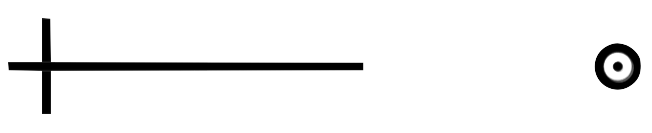
\includegraphics[width=14cm]{img/penalty.png}
  \caption{ペナルティ計測用コース} \label{fig:penalty}
\end{figure*}

予備競技会では,ライントレーサを作製して決められたコースのタイムトライアルを行う.ライントレース用のコースは図~\ref{fig:linetrace}に示す.上の図~\ref{fig:training}はトレーニング用コースを示し,このトレーニングコースよりも半径の小さなカーブはない.実際のコースは下の図~\ref{fig:yobi}に示し,このコースは予備競技会当日に発表される.

\begin{figurehere}
  \centering
  \begin{subfigure}{0.45\textwidth}
    \centering
    
\includegraphics[width=4.5cm,angle=270]{img/training.pdf}
    \caption{トレーニング用コース} \label{fig:training}
  \end{subfigure}
  \begin{subfigure}{0.45\textwidth}
    \centering
    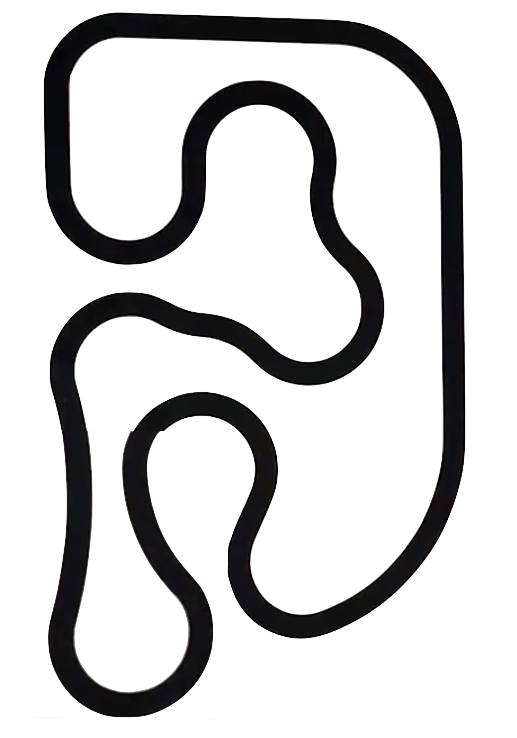
\includegraphics[width=3.8cm,angle=90]{img/yobitaikai.png}
    \caption{予備大会用コース} \label{fig:yobi}
  \end{subfigure}
  \caption{ライントレース用コース}\label{fig:linetrace}
\end{figurehere}

開発の段階では,トレーニングコースでしかテストできないが,トレーニングコースを右回り・左回りのいずれも確実に周回でき,さらに円のコースでも同様に周回できれば,実際のコースでも周回できると考えられる.

予備競技会では,ライントレースだけでなく,目的地に確実に到着できるかどうかも確認される.ライントレースのタイムトライアル後に,ソフトウェアを切り替えることは可能であるが,ハードウェアには一切手を加えることなく,図~\ref{fig:penalty}のようなペナルティ計測用コースを左から右に向かって走行する.コースのサイズは,左の十字の中心から的の中心までが1,500mmとなっている.停止した位置が的の中心からずれるにしたがって,ライントレースのタイムに最大20\%のペナルティが加えられる.

予備大会当日は,コースが発表された後,時間計測の前に,実際のコースに合わせて調整する時間が設けられており,必要に応じてハードウェアやソフトウェアを修正できる.

\subsection{戦略}
この予備大会で好成績を残すためには,ライントレースを行えるだけでなく,目的地へ確実に到着する技術も必要となる.第2節に書いたように,本競技会において,コーナー(カーブ)で差が付きやすいと考えた.ハードウェアの面では,センサーからの値を確実に習得し,その値をすぐにタイヤへ反映できるようにすることと,どんなカーブでも素早く曲がることができるようにすることを設計目的とする.ソフトウェアの面では,センサー値を用いて正確にモーターのパワー比率を制御する方法,直進できるように両方のモーターの回転数を保持するための方法や,目的地を認識して確実に停止する方法の3つを実装しなければならないと考えた.これらのハードウェアとソフトウェアの戦略を実現しようとした結果を以下に説明する.また,本課題の開発スケジュールは,付録~\ref{apdix:schedule}に表示した2018/10/4から2018/10/25までのスケジュールである.

\subsection{ハードウェア}%魚躬,本間:設計の目的,結果(機体の仕様).問題点,克服した点,工夫した点など.
4.1節に説明した戦略を意識しながら作製したハードウェアを図~\ref{fig:linetracer}に示す.また,図からは読み取れない仕様を表~\ref{tab:spec1}に示す.

\begin{figurehere}
  \centering
  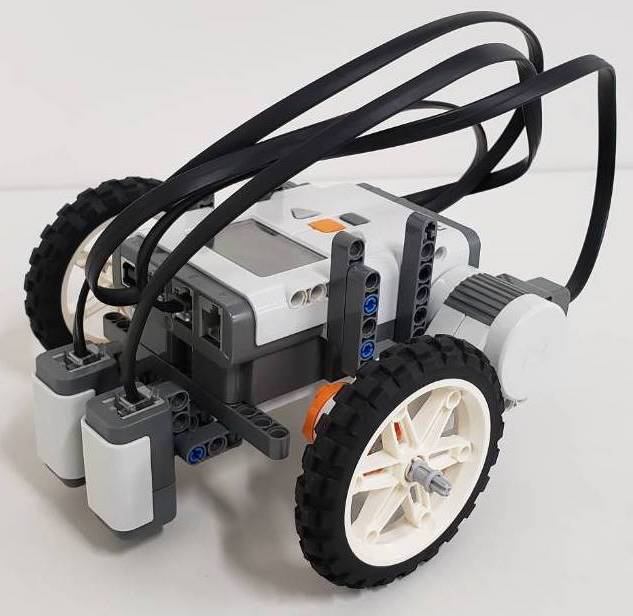
\includegraphics[width=5cm]{img/linetracer.jpg}
  \caption{予備競技会で作製した機体} \label{fig:linetracer}
\end{figurehere}

\begin{center}
\begin{tablehere}
	\caption{予備大会で作製した機体の仕様}
	\label{tab:spec1}
	\begin{tabular}{c|c}
	\doubleRule
	重量 & 600 [gr] \\\hline
	部品数 & 52個 \\\hline
	センサーとタイヤ間の距離 & 10 [mm]\\\hline
	センサーの地面からの距離 & 9 [mm]\\\hline
	センサー間の距離 & 32 [mm]\\\hline
	タイヤ間の距離 & 145 [mm]\\\hline
	\bottomrule
	\end{tabular}
\end{tablehere}
\end{center}

工夫した点は重量,センサーの位置,タイヤの位置,センサーとタイヤ同士の位置,全体のバランスの5点である.重量は部品の数をサンプルハードウェアの110個から52個に減らしたことによって745 [gr]から600 [gr]まで軽量化することができた.この軽量化を実現できたのはハードウェア全体の安定性を支える重要な部品にのみ丈夫で重い部品を扱い,それ以外の部分には極力部品を付けない,または軽い部品を使うように工夫したからである.

センサーの位置について説明する.まずセンサーはライトセンサーとカラーセンサーの2つがあり,この2つの距離をサンプルの40 [mm]から32 [mm]に近づけることで車線に合わせて常にグレーの値が良い撮れるように工夫した.また,センサーの地面からの高さをサンプルの14 [mm]から9 [mm]にしたことでよりセンサーの値を確実に取得し,PID制御がしやすくなるようにした.タイヤの位置は,タイヤ同士の距離を145[mm]に近づけることで曲がるときによりインコースで曲がることができるように工夫した.センサーとタイヤ同士の位置は,センサーとタイヤの距離を10 [mm]に近づけたことでセンサーから読み取った値をすぐにモーターに反映させるkとができるように工夫した.全体のバランスは,ハードウェアの後方にボール付きのピンをつけたことで全体の重心をタイヤの近くにすることができた.これによって走行中にハードウェアが滑ってしまうことを防ぎ,より線に沿った走行が行えるようになっている.

\subsection{ソフトウェア}%鈴丸,原田:書いたプログラムの概要(アルゴリズム)・目的,使い方.結果の問題点,克服した点,工夫した点など.
\subsection*{【ライントレース】}
ライントレースのプログラムについて説明する.ライトセンサーとカラーセンサーを一つのセンサーで扱う方針にした.まず線をまたいでキャリブレーションを行い,ライトセンサーの値からカラーセンサーの値を引いてターゲット値を決める.このターゲット値と実際の走行中の値との誤差で左右どちらに曲がるのか決定する.それに加えて,センサー値の変化が連続的であるため,値の大きさでカーブの半径を予測でき,それに対する適切なパワーをモーターに与えることができる.つまり,センサー値とパワー値が比例関係にあり,センサー値の変化や累積された誤差に基づいて,より正確なパワー制御ができる.これをPID制御という.ただし,PID制御は適切な定数を与えなければまともに機能しないため,調整が必要になった.そのため,画面上でPID制御のそれぞれの定数を変更できるような関数を作成した.これにより調整にかかる時間を短くした.さらに,本番のコースを試走しながら定数の変更をでき,より本番のコースに最適な定数を調整することが可能となった.しかし,予備競技会の本番では調整が十分ではなかったため直線でジグザグ走行したり,脱線したりしてタイムロスをしてしまった.

次にカーブを曲がる際の工夫点を説明する.小さなカーブを曲がるときには曲がった後でセンサーの位置が線からずれないように,かつ素早く曲がれるように,逆回転するようにした.円内にあるタイヤが逆転してセンサーが線からずれずに素早く曲がることができるようにした.その結果,練習用の円のコースで素早くかつ正確にカーブを曲がることができた.しかし本番では,曲がりすぎたりしてうまくいかなかった.

\subsection*{【ペナルティ計測】}
状態管理で5つの状態に分けるプログラムを書いた.それは左の十字から右の二重円に向かって黒いライン上を走る状態,白い領域を走る状態,二重円の外側の黒い線を感知した状態,円内の白い領域を感知した状態,円の中央の黒円を感知した状態に分けた.しかし,これには問題があって,1つでも状態を通らないと永遠に最後の状態にはたどり着けないというものだったり,円の線をしっかり感知するには車体のセンサー2つともがしっかり線を認識しなければならないといけないという内容のものであった.そこで, Stateを極端に減らし,精度を上げるために十字から円までの移動はセンサーを使わず,左右のモーターでPI制御をして移動するようにした.その時のプログラムを付録~\ref{apdix:linetracer}に示す. 

結果的に練習時にはこれで円の中央に止まることができたのだが本番では何故か中央の黒円を素通りしていったのだ.この原因は2個目の黒円到達後に\texttt{State}を初期値であるNoneにしているため\texttt{do while()}文がまた最初から走査されてしまい,結果的にそのまま走り抜けてしまったということであった.ここでStateを\texttt{StateNum}に変えておけばちゃんと止まったと考えられる.結果的にイージーミスが大きなミスにつながってしまったためコードを書く時の良い教訓になった.

\subsection{考察}%全員:パーフォマンスを評価して,何が成功したか何が失敗したかとその理由.失敗に関しては改善方法などを挙げる.%バッグでロボットが止まらない,PID定数の調整,
ライントレースにおいて直線でジグザク走行してしまったのがタイムロスとなってしまった.これはPID制御の定数の調整がうまくいかなかったと考えられる.また,全体的に作業の時間配分が甘かったため,メンバー間の作業量を調整することが課題となった.

\section{もの集め競技会}
\begin{figure*}[!t]
  \centering
    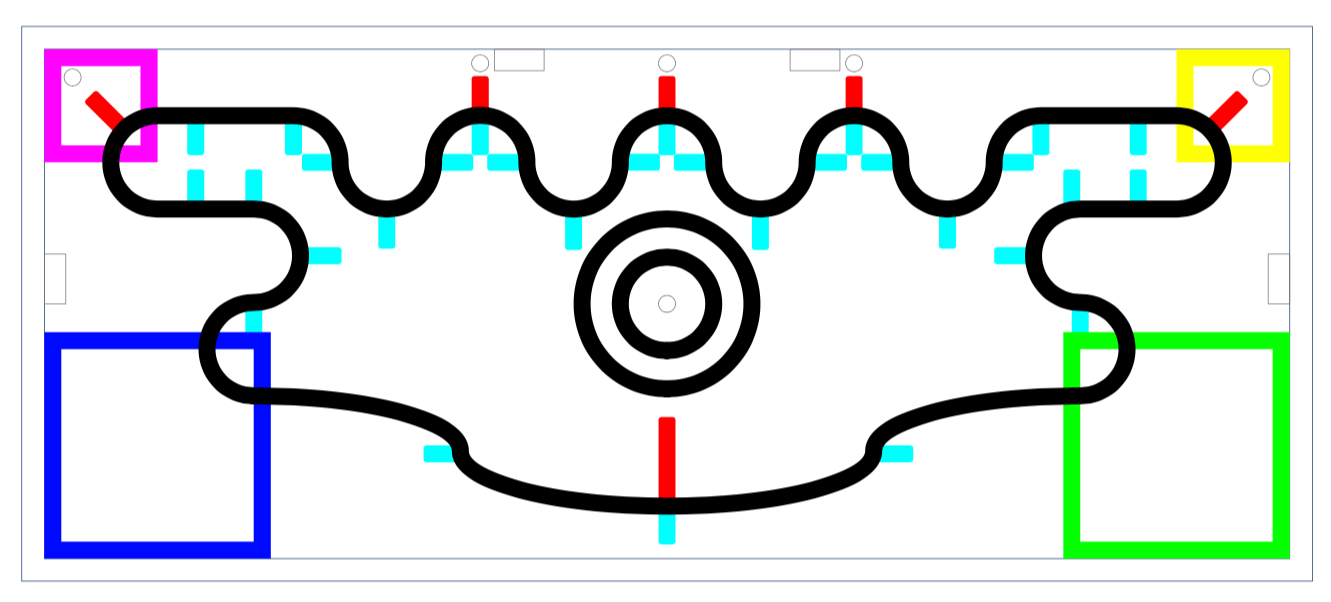
\includegraphics[width=14cm]{img/monocourse.png}
  \caption{もの集め競技会のフィールド} \label{fig:monocourse}
\end{figure*}

もの集め競技会は,図~\ref{fig:monocourse}に示すフィールド上に置かれたオブジェクトを集めることで得点を得て,合計得点を競い合うゲームである.フィールド右下(決勝の競技会では右下と左下の両方)の四角がベースであり,ロボットはここから出発させる.ロボットは自律的に動作しなければならない.ただし,ベース内は特別であり,ロボットの調整や修理が可能である.ロボットが自律的にベースに戻れない時には手で運ぶことも可能だが,この場合には得点にペナルティが課される.

ゲーム終了時に,オブジェクトがフィールド4隅の四角形の内側の部分に触れていれば,得点を獲得できる.それぞれの四角には倍率が決められており,オブジェクトによる得点はさらに増す.

第1弾の予選競技会と第2弾の決勝競技会は,基本的には同じ競技を行う.ただし,一部だけ「競技ルールの仕様変更」を行う.つまり,第1弾と第2弾では競技が若干異なる.あらかじめ,仕様変更に耐えられるような設計をしておくことが望ましい.

%\subsection{戦略}
\subsection{ハードウェア}%魚躬,本間:設計の目的,結果(機体の仕様).問題点,克服した点,工夫した点など.
シンプルさに注目して設計を進めた.簡単な部品の取り外しなどが可能であったことにより効率的に作業を進める事ができた.
\subsection*{【予選】}
もの集めの予選競技会では,図~\ref{fig:monorobot1}ソフトウェアとハードウェアの開発を両立するためにNXTは置くだけで本体に設置できるようにした.これにより,NXT本体の取り外しの自由度が高まった.本体の構造としては,ステージの特性を考察してカラーセンサーを本体の左部分に設置するようにした.また,アルゴリズム設計の負担を減らすよう,シンプルな動作でオブジェクトを回収できるような本体設計を目指して,アーム部分は低く設計した.これにより,オブジェクトに直進するだけでオブジェクトを回収できるようにした.シンプルに,最低限の動作を行えるような本体設計をめ実現した.しかし,壁際でのアームの上下運動の際にアームが壁に引っかかったり,オブジェクトに対して進入する角度によっては上手く回収できないという問題もあった.

\begin{figurehere}
  \centering
  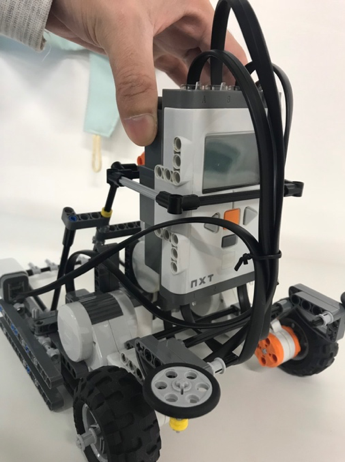
\includegraphics[width=5cm]{img/monorobot1.png}
  \caption{もの集めの予選競技会で作製した機体}
  \label{fig:monorobot1}
\end{figurehere}

\subsection*{【決勝】}
もの集めの決勝競技会では,予選競技会における本体の問題点の改善とさらなる改良を目指した.まず,NXTを本体の一部として組み込む設計に変えた.NXTにもパーツを拡張する部分があるので本体拡張の自由度が上がった.次に,アームなどの本体の前方部分を大幅に改良した.本体の両側に設置したタッチセンサーを誤作動なく反応させるために,タッチセンサーの先端から前方に向けて拡張している部分の強度を上げた.これにより, タッチセンサーの誤作動を防ぎながらオブジェクト回収にも役に立つようになった.また,第一回で課題となった壁際でのアームの動作において引っ掛かりが生じてしまうことについては,第一回ではアームの根元が本体上部にある事が原因であったと考えたのでそれを地面に近くなるよう設計し直した.これにより壁際でアームが引っかかる事がなくなった.

\subsection{ソフトウェア}%鈴丸:書いたプログラムの概要(アルゴリズム)・目的,使い方.結果の問題点,克服した点,工夫した点など.
\subsection*{【予選】}%カラーセンサー,タスク管理,wrapper関数
第1弾の物集め競技会では1つも物を集めることはできなかった.以下に原因を示す.
\begin{enumerate}
   \item タスク管理,センサー処理などの細部の動作に時間をかけすぎた.
  \item 旋回用の関数がなかったため, 車体の方向を変える動作に柔軟性が足りなかった.
  \item 実験回数が足りなかった.
\end{enumerate}
結局基本の軸となるアルゴリズムよりも細部の機能に時間をかけすぎたたため物集め本体のアルゴリズムにかける時間が足りなくなり中途半端な結果になってしまったと考えられる. 

次に具体的な第1回目の物集め競技会のアルゴリズムを説明する.物集め全体のアルゴリズムはハードコーディングで技術的に説明することはなにもしていないためこのアルゴリズムで使われている\texttt{mov\_func()}関数と\texttt{arm\_func()}関数について説明する.\texttt{arm\_func()}関数は第1引数にモーターのパワー,第2引数に上げ下げの\texttt{degree}を受け取る.内部ではDEGの正負でアームの上げ下げの区別し,モーターの回転数が\texttt{DEG}の絶対値を超えたらモーターを止めることでアームを動かす仕組みになっている.また,アームの上げ下げ角度をディスプレイに表示する機能も付いている.

第1引数にマスターモーターのパワーを第2引数に曲がり具合を第3引数にどのぐらいの回転数\texttt{mov\_func()}を実行するかという値が与えられている.第2引数が0であればまっすぐに進み,正であれば右寄り,負であれば左寄りというようになっている.内部ではPID制御によってマスターモーターとスレイブモーターのパワーを切り替えることで与えられた値に準ずる正確な走行が可能となる.また,デバッグ用としてディスプレイに現在の左右のモーターの回転数を出力する機能も付いている. 

次に,競技会では使用しなかったが,色センサーの判定アルゴリズムについて説明する.フィールド上の色は赤,緑,青のモニターの3原色に加えて,白,黒,および,シアン,マゼンタ,黄の印刷物の3原色である.このため,判定方法は,色を混ぜれば混ぜるほど明るくなるといった加法混色と,色を混ぜれば混ぜるほど暗くなる減法混色の原理を利用した.アルゴリズムはまず,各RGBの閾値を実際のフィールドで計測することにより決定する.次に,各RGB値が閾値よりも高ければ1,それ以外の場合は0を出力する関数を用意する.そのRGBの3ビットのビットパターンで色を判定する.例えば,(0,1,0)と出力されたら緑と判定し,(1,1,0)と出力されたら黄と判定し,(1,0,1)と出力されたらマゼンダと判定する.この方法は実際のセンサー値を基に閾値を決定しているため色を間違えることがほとんどないことがメリットである.付録~\ref{apdix:mono}に表示したソースコード~\ref{ls:colorSense.c}のように,ビット演算を使用して色を計算した.閾値はソースコード上の\texttt{COL\_THRES}であり, 実際の競技場の色を調べながら決めることで正確な判定ができるようになった.この関数を実際に利用するために,タスク間通信を行うための方法の1つであるイベントフラグ処理が必要となる.しかし,タイムティックを正しく提供できないため,イベントフラグによる通知が正しく動作しなくなると考えられる.デバッグ時間があまりなかったため,この関数を使用しないことになったが,この関数だけのテストでは100\%でフィールドの色を全て正しく判定できた.

\subsection*{【決勝】}%ボール回収方法,中タイヤやT字ブロックなど
第2弾の物集め競技会では第1弾の失敗を反省し作業に取り掛かったが,第2弾でも物はあまり集められなかった.フィールドの少しの環境変化でうまく動作しないことが多くあったという新たな原因が生じた.

結果的に練習環境では成功することもあったが失敗することもあり不安定な状態で競技に臨んだ結果,本番環境ではうまくいかなかったのが一番の敗因だろう.次に第1弾の競技会では実装されていなかった\texttt{steering()}関数について説明する.\texttt{steering()関数}は第1引数に左回転か右回転かを判定するための\texttt{direction}を受け取り,第2引数に旋回するときに動かすモーターの回転数を受け取る.内部では\texttt{direction}の値によって動かすモーターと止めるモーターを決め,動かすモーターが\texttt{angle}以上になったら旋回終了という単純なアルゴリズムになっている.

\texttt{mov\_func()},\texttt{arm\_func()},\texttt{steering()}はどれも関数が呼ばれるタイミングによって回転数も大きく変わるためある程度の誤差が生じるためその誤差の対処もしておくようするべきであったと考える.

\subsection{考察}%全員:パーフォマンスを評価して,何が成功したか何が失敗したかとその理由.失敗に関しては改善方法などを挙げる.%ロボットが軽すぎたため,タイヤの空回り.3倍矩形を狙わずに,2倍のままにボールを落とす戦略など
練習コースではうまくいったが本番のコースではうまくいかなかった.本番コースでの試走でプログラムの定数の調整をする必要があった.また,実際に作製したロボットがシンプルで軽量過ぎたため,平らではないフィールドではタイヤが空回りしてしまい,定数によって指定された目的地からずれるようになると考えられる.

両方のもの集め競技会ではロボットがものを回収できないというわけではなく,目的となる矩形に運ぶことができないことが低い得点の原因と考えられる.対応策として,途中で戦略を変更可能なロボットを準備することが挙げられる.具体的に,実際の競技会ではボールを落とすことができたため,得点の高い矩形を狙わずに落とした矩形にオブジェクトを置く戦略をメニューから選択できるようにすれば良かったと思われる.そうすれば獲得できる点は下がるが,成功する確率が上がるため,現在の結果よりも良い結果が得られる可能性も上がる.また,一定時間が経った後,ロボットを自動的にベースに戻るルーチンを準備すれば,試技中に目的地に到達できない場合でもベースに戻れるため,手で触ったペナルティを削除することができると考えられる.

\section{プレゼンテーション大会} %原田:評価基準を基に良いプレゼント手法とは?
プレゼンテーションの5つの評価基準は以下に示す.
\begin{enumerate}
\item 内容\\ チームのアイディア,独自性は明確かどうか,技術的工夫が詳細に述べられているかを評価する項目である.
\item 構成\\ 発表の流れはしっかりした論理展開か,結果に対する考察がなされているかといった点を評価する項目である.
\item スライド\\ スライドの文字の大きさは適切か,図表の数や大きさは適切かといった点がこの項目の評価対象である.
\item 発表\\ 明瞭に聞き取りやすい話し方か,聞き手を見て説明できたか,質疑応答は的確かを評価する項目である.
\item 発表時間\\ 5分という発表時間制限が守られたかどうかを評価する項目である.
\end{enumerate}
以上の評価基準は,研究会等で科学界における一般的な評価基準であり,これを全て満たせば良い発表ができると考えられる.

実験期間中にプレゼンテーション大会が2回行われた.初回のプレゼンテーション大会では,予備競技会の結果を踏まえたプレゼンを行った.自身のチームのロボットのソフトウェアとハードウェアの優れた点,工夫した点をプレゼンするとともに,競技会で分かった問題点や弱点と,それらを克服するための改善策などについて発表した.プレゼンテーションの結果は学生6位,教員・TAは9位で総順位は7位となった.評価については内容と構成,発表時間に関しては良かったが,スライドと発表が比較的に低かった.原因としては,他のチームと比べスライドの文章が長くて簡潔ではなかったことが挙げられる.また,発表原稿を覚えていなかったため,聞き手の方を向かずに発表していたため発表の項目が悪かったと考えられる.他の項目についてはハードウェアの設計に関して写真を使って説明できたこと,ソフトウェアの改良した際の動画等を載せていたため根拠のある発表ができた.

2回目のプレゼンテーション大会は,もの集め競技会予選・決勝に関するプレゼントを行なった.単にロボットに設計やソフトウェアについて述べるだけでなく,チームとしての戦略も発表した.また,1回目のプレゼンテーションの評価を踏まえた発表となるように心がけた.プレゼンテーションの結果は学生が8位,教員・TAが11位で総順位は11位となった.評価については初回のときよりも構成,発表の項目が下がっていた.構成において競技会で使用しなかった方法の説明が長かったため,評価が下がったと考えられる.発表に関しては発表原稿を暗記していたが,話し方が単調,早口で聴衆に聞き取りづらかったというコメントが多く,初回のプレゼントと同様に発表の項目が改善しきれなかった.一方,「ハードウェアの工夫点が面白い」,「スライドが見やすい」,「説明が分かりやすい」というコメントがあり,初回のプレゼンの悪かったスライド項目は改善できていた.

\section{Wikiページ} %原田,本間:WIkiページの目的,何を記載したか,どの手法で編集したか
Wikiページの目的はチームの活動を受講生全員に広報することとプレゼン資料の作成する際などに今までの活動を確認できるようにすることである.ページの作成方法は,wordファイルで内容を作成し,wordファイルからhtmlへ変換するソフトを用いて変換し,moodle上のWikiページに出力した.内容はメンバーの役割分担,毎週のチームの目標とその日に行ったチームの活動内容等を細かく記載した.


\section{全体の考察とまとめ}%全員:各自,自分が書いた節の考察からまとめる
全体的にプログラムの定数の調整に十分な時間が割けなかった.メンバー間の作業量の調整がうまくいってなかったと考えられる.また,最初から細部に集中して多くの時間が取られてしまったことも失敗の原因と考えられる.今回のように時間が限られている開発の中ではまず競技全体のアルゴリズムをハードコーディングでも完成させることで最低限のプロダクトを用意し,精度を上げる過程で細部のセンサー処理などの実装にとりかかるべきであったと思われる.自分たちはチーム内でのタスク管理が少し曖昧だったためその辺りの認識をそろえる必要があったと考えた. 

\section{感想}%全員:各自,自分の感想を書く(目的に書いてあったものを参考にすると良いかも)
今回の実験を通してメンバーでのプロジェクト開発の難しさやプログラムに関する知識が乏しいことが実感できた.しかし,メンバー間で意見を言い合い協力できたことは良かった.結果が良くはなかったが,チームメンバの全員がこのチームで良かったと思っている.

本実験を通して,組み込みシステムのプログラミングを体験することができた.githubのようなチームでソースコードを共有するためのプラットフォームの使い方に関しても勉強できた.最後に,実際にプレゼンテーションを行ったため,良いプレゼンテーションの仕方も学ぶことができた.

%%====			Bibliography			====%%
\begin{thebibliography}{9}

\bibitem{textbook}
2018年度情報画像実験\rom{3}テキスト

\bibitem{toppers}
ETロボコン向けRTOS活用コンテンツ,\url{https://www.toppers.jp/etrobo-jsp.html}

\bibitem{osek}
nxtOSEK/JSP,\url{http://lejos-osek.sourceforge.net/jp/index.htm}

\bibitem{osekapi}
nxtOSEK C API,\url{http://lejos-osek.sourceforge.net/ecrobot_c_api_frame.htm}

\bibitem{itron}
$\mu$ITRON4.0仕様 Ver. 4.02.00,\url{http://www.ertl.jp/ITRON/SPEC/FILE/mitron-402j.pdf}

\end{thebibliography}
\noindent (URLは2019年2月現在)
\end{multicols*}

\newpage
\begin{appendices}
\section{チームのスケジュール} \label{apdix:schedule}
本実験でのチームのスケジュールは表~\ref{tab:sched}に示す.この表に,各実験日のチーム全体の目標,その目標を達成するために行った作業やその作業の達成度を表示する.
%\begin{table}[!h]
%\centering
%\caption{チームのスケジュール}
%\label{tab:sched}
%  \begin{tabular}{c|M{6cm}|M{6.5cm}}
%  \doubleRule
%    日付 & 目標 & 行った作業(達成度) \\\hline
%  \bottomrule
%  \end{tabular}
%\end{table}

\begin{center}
\begin{longtable}{c|M{6cm}|M{6.5cm}}
\caption{チームのスケジュール}
\label{tab:sched} \\

\doubleRule 日付 & 目標 & 行った作業(達成度)\\\hline 
\endfirsthead

\multicolumn{3}{c}%
{{\bfseries \tablename\ \thetable{} -- 前ページの続き}} \\
\toprule 日付 & 目標 & 行った作業(達成度)\\\hline
\endhead

\hline \multicolumn{3}{r}{{次のページに続く}} \\
\endfoot

\bottomrule
\endlastfoot

    2018/10/4 & サンプルロボットの動作を確認してライントレーサの基本知識を取得する & 
    \begin{enumerate}
    \item サンプルロボットの組み立てとサンプルプログラムのインストール(100\%)
    \item 動作確認とライントレーサ原理の調査(100\%)
    \item 改良方針を決める(100\%)
    \end{enumerate}\\\hline
    2018/10/11 & サンプルプログラムを改良してテストコースで9.5秒以下に走行できるようにする &
    \begin{enumerate}
    \item 直進して目的地に停止するための制御の実装(60\%)
    \item ライントレーサの制御の実装(50\%)
    \end{enumerate}\\\hline
    2018/10/18 & テストコースで9秒以下に走行できるようにロボットを軽量化する &     
    \begin{enumerate}
    \item ライントレーサ制御の改良(70\%)
    \item 不必要なパーツを機体から外す作業(50\%)
    \end{enumerate}\\\hline
    2018/10/25 & ペナルティ計測で目的地に停止できるようにする &
    \begin{enumerate}
    \item ペナルティ計測用のアルゴリズムの実装(50\%)
    \item ハードウェアの軽量化(100\%)
    \end{enumerate}\\\hline
    2018/11/8 & 予備大会でロボットが30秒以内に完走でき,ペナルティが10\%以内にする &
    \begin{enumerate}
    \item ライントレーサの制御に使用される定数の調整(100\%)
    \item ペナルティ計測に使用される定数の調整(70\%)
    \end{enumerate}\\\hline
    2018/11/15 & 発表大会の資料を完成させ,もの集めの基本的な機能を実現する &
    \begin{enumerate}
    \item 発表の準備(80\%)
    \item タッチやカラーセンサーから値を取得するための機能の実装(60\%)
    \item アーム仕組みの開発(70\%)
    \end{enumerate}\\\hline
    2019/11/22 & 走行時間を考慮せずに,コースにある物を全て回収できるようなもの集めのロボットを完成させる & 
    \begin{enumerate}
    \item 走行全体のアルゴリズムの開発(60\%)
    \item 機体全体の組み立て(60\%)
    \end{enumerate}\\\hline
    2018/11/29 & もの集めロボットver1.0を完成させて実験を行い,その結果に基づいて改善すべき点を調べる &
    \begin{enumerate}
    \item ディスプレイを用いたデバッグ機能の実装(60\%)
    \item 組み立てた機体で実験して,改善できる点の調査(100\%)
    \end{enumerate}\\\hline
    2018/12/6 & もの集めの予選競技会で8位以上を収められるロボットを完成させる&
     \begin{enumerate}
    \item ものを個別に集めるためのアルゴリズム開発(30\%)
    \item ロボットの剛体性を向上させる作業(70\%)
    \end{enumerate}\\\hline
    2018/12/13 & もの集めの予選競技会の様子を見て,自分チームや他のチームの長所と短所を調査する &
    \begin{enumerate}
    \item 大会中にハードウェアを保守,改良する作業(90\%)
    \item ものを個別に集めるためのアルゴリズムのパラメータ調整(80\%)
    \end{enumerate}\\\hline
    2018/12/20 & 青ベースまたは緑ベースから開始して80秒以内に全てのボールを3倍の矩形に運ぶためのロボットを設計する &
    \begin{enumerate}
    \item 青ベースと緑ベースのアルゴリズムを分割する作業(90\%)
    \item 機体の剛体性とアームの制御しやすさを向上させるための作業(85\%)
    \item タスク管理とイベントフラグの実装(80\%)
    \end{enumerate}\\\hline
    2018/12/27 & 青ベースまたは緑ベースから開始して80秒以内に全てのボールを3倍の矩形に運ぶためのロボットを完成させる &
    \begin{enumerate}
    \item 発表の準備(100\%)
    \item ボールを集めるためのアルゴリズムのパラメータ調整(80\%)
    \item コースでの実験結果を基に,アームの改良作業(100\%)
    \end{enumerate}\\\hline
    2019/1/10 & 40秒以内に2重タイヤの中タイヤとT字ブロックを2倍矩形に回収するためのロボットを完成させる &
    \begin{enumerate}
    \item 2重タイヤの中タイヤとT字ブロックを集めるためのアルゴリズム開発(100\%)
    \item 中のタイヤを釣り上げるためのアーム開発(100\%)
    \item T字ブロックを運ぶためのアーム開発(100\%) 
    \end{enumerate}\\\hline
    2018/1/17 & ボールを回収するためのアルゴリズムと,中タイヤとT字ブロックを回収するためのアルゴリズムを合成させ,最終アルゴリズムを完成させる & \begin{enumerate}
    \item 今まで開発したアルゴリズムを統合させる作業(90\%)
    \item Wikiページの更新(100\%)
    \item アルゴリズムの実験結果に基づいたハードウェアの改善作業(100\%) 
    \end{enumerate}\\\hline
    2018/1/24 & もの集めの決勝競技会で最善を尽くし,最終チームレポートにまとめる作業を始める &
    \begin{enumerate}
    \item アルゴリズムのパラーメータ調整やハードウェアの保守(100\%)
    \item 最終チームレポートの共有ファイルを作成して実験で行った作業をまとめる(100\%)
    \end{enumerate}\\\hline
\end{longtable}
\end{center}
\clearpage

\section{予備競技会で作成したソースコード} \label{apdix:linetracer}
予備競技会のペナルティ計測のためのプログラムをソースコード\ref{ls:penalty.c}に示す.ただし,このソースコードは説明に関連する部分だけを示し,他の部分は中略されている.
\inputcode[label=ls:penalty.c]{src/penalty.c}
\clearpage

\section{もの集め競技会で作成したソースコード} \label{apdix:mono}
もの集め競技会のためのプログラムをソースコード以下に示す.ただし,これらのソースコードは説明に関連する部分だけを示し,他の部分は中略されている.
\inputcode[label=ls:arm_func.c]{src/arm_func.c}
\inputcode[label=ls:mov_func.c]{src/mov_func.c}
\inputcode[label=ls:colorSense.c]{src/colorSense.c}
\inputcode[label=ls:steering.c]{src/steering.c}
\clearpage

%\section{もの集め競技会決勝で作成したソースコード} \label{apdix:mono2}
%\inputcode[label=ls:.c]{src/jouga.c}
%\inputcode[label=ls:.h]{src/jouga.h}

\end{appendices}

\end{document}
